\documentclass[12pt,a4paper]{article}

\usepackage[margin=0.68in]{geometry}
\usepackage[T1]{fontenc}
\usepackage[utf8]{inputenc}
\usepackage{lmodern}
\usepackage{amsmath,amssymb}
\usepackage{graphicx}
\usepackage{booktabs}
\usepackage{array}
\usepackage{enumitem}
\usepackage{xcolor}
\usepackage[most]{tcolorbox}
\usepackage{titlesec}
\usepackage{fancyhdr}
\usepackage{hyperref}
\usepackage{microtype}
\usepackage{listings}
\usepackage{parskip}

\hypersetup{colorlinks=true,linkcolor=blue!50!black,urlcolor=blue!50!black,pdftitle={UEC-310 Assignment Report},pdfauthor={Rishit}}

\definecolor{titleblue}{HTML}{1F4E8C}
\definecolor{accent}{HTML}{E26D3A}
\definecolor{teal}{HTML}{1B9E77}
\definecolor{softblue}{HTML}{EAF2FF}
\definecolor{softgreen}{HTML}{EDF7ED}
\definecolor{softyellow}{HTML}{FFF4D8}
\definecolor{softgray}{HTML}{F4F4F2}
\definecolor{softline}{HTML}{D9DDE3}
\definecolor{codebg}{HTML}{F7F8FA}

\pagestyle{fancy}
\fancyhf{}
\lhead{UEC-310 Information and Communication Theory}
\rhead{Assignment Report}
\cfoot{\thepage}
\setlength{\headheight}{14pt}

\titleformat{\section}{\large\bfseries\color{titleblue}}{}{0pt}{}
\titleformat{\subsection}{\normalsize\bfseries}{}{0pt}{}
\titlespacing*{\section}{0pt}{0.7em}{0.35em}
\titlespacing*{\subsection}{0pt}{0.45em}{0.2em}

\setlist[itemize]{leftmargin=1.4em,itemsep=0.1em,topsep=0.15em}
\setlist[enumerate]{leftmargin=1.4em,itemsep=0.1em,topsep=0.15em}

\newtcolorbox{formulaBox}{colback=softgray,colframe=softline,boxrule=0.5pt,arc=2mm,left=2mm,right=2mm,top=1mm,bottom=1mm}
\newtcolorbox{blueNote}{colback=softblue,colframe=softblue,boxrule=0pt,arc=2mm,left=2mm,right=2mm,top=1mm,bottom=1mm}
\newtcolorbox{greenNote}{colback=softgreen,colframe=softgreen,boxrule=0pt,arc=2mm,left=2mm,right=2mm,top=1mm,bottom=1mm}
\newtcolorbox{yellowNote}{colback=softyellow,colframe=softyellow,boxrule=0pt,arc=2mm,left=2mm,right=2mm,top=1mm,bottom=1mm}

\lstdefinestyle{py}{
  language=Python,
  backgroundcolor=\color{codebg},
  basicstyle=\ttfamily\footnotesize,
  keywordstyle=\color{titleblue}\bfseries,
  commentstyle=\color{teal!70!black},
  stringstyle=\color{accent!80!black},
  showstringspaces=false,
  frame=single,
  rulecolor=\color{softline},
  frameround=tttt,
  xleftmargin=0pt,
  xrightmargin=0pt,
  aboveskip=0.4em,
  belowskip=0.3em,
  columns=fullflexible,
  keepspaces=true,
  breaklines=true
}

\begin{document}

% ---------------- TITLE PAGE ----------------
\begin{titlepage}
\thispagestyle{empty}
\centering
\vspace*{1.3cm}
{\large \textbf{Thapar Institute of Engineering and Technology}}\\[0.25cm]
{\normalsize Electronics and Communication Engineering Department}\\[1.4cm]

{\Huge \bfseries UEC-310}\\[0.2cm]
{\LARGE \bfseries Information and Communication Theory}\\[1.2cm]

\begin{tcolorbox}[enhanced,boxrule=0pt,colback=softblue,width=0.88\textwidth,arc=3mm]
\centering
{\Large \bfseries Assignment Report}\\[0.25cm]
Reliable Data Transmission in a Satellite Communication System
\end{tcolorbox}

\vspace{1.6cm}
\renewcommand{\arraystretch}{1.35}
\begin{tabular}{>{\bfseries}p{4.2cm}p{6.8cm}}
Student Name & Rishit Bhanot \\
Tools Used & Python, NumPy, Matplotlib, Seaborn \\
\end{tabular}
\vspace{1.6cm}

\begin{tcolorbox}[enhanced,boxrule=0pt,colback=softblue,width=0.88\textwidth,arc=3mm]
\centering
Submitted to : Dr. Geetanjali Chandwani Manocha
\end{tcolorbox}
\vspace{1.6cm}

\begin{tcolorbox}[enhanced,boxrule=0pt,colback=softyellow,width=0.88\textwidth,arc=3mm]
\centering
\href{https://github.com/rishitbhanot1/ict_assignment_uec310}{GitHub Repository : https://github.com/rishitbhanot1/ict\_assignment\_uec310}
\end{tcolorbox}

\vfill
\begin{tcolorbox}[enhanced,boxrule=0pt,colback=softgray,width=0.9\textwidth,arc=2mm]
\small
This report addresses the problem of reliable transmission of environmental sensor data in a satellite communication system, where long-distance propagation and atmospheric disturbances introduce noise into the channel. It combines the analytical study of source entropy, coding efficiency, and Binary Symmetric Channel capacity with a reproducible simulation-based evaluation of bit errors and channel performance under noisy conditions.
\end{tcolorbox}

\vfill
\end{titlepage}

\small

% ---------------- PAGE 2 ----------------
\section*{Problem Statement}
Reliable Data Transmission in a Satellite Communication System: A satellite 
communication company is transmitting environmental data from remote sensors on Earth to 
a ground station. Due to long-distance transmission and atmospheric disturbances, the 
communication channel is noisy, leading to possible data corruption.

\section*{Part A: Analytical Tasks}

\subsection*{Q1. Entropy and Source Coding}
Given:
\begin{itemize}[leftmargin=2em]
    \item Probability of bit `1': $P(1)=0.7$
    \item Probability of bit `0': $P(0)=0.3$
\end{itemize}

\begin{formulaBox}
\[
H(X) = -p(1)\log_2 p(1) - p(0)\log_2 p(0)
\]
\end{formulaBox}

\begin{enumerate}[leftmargin=2em,label=\arabic*.]
    \item Substitute the given probabilities:
    \[
    H = -0.7\log_2(0.7) - 0.3\log_2(0.3)
    \]

    \item Using approximate logarithm values:
    \[
    H = -0.7(-0.5146) - 0.3(-1.7370)
    \]

    \item Simplify:
    \[
    H = 0.3602 + 0.5211
    \]
\end{enumerate}

\[
\boxed{H(X)=0.8813\ \text{bits/symbol}}
\]

\begin{blueNote}
\textbf{Interpretation:} Each source symbol carries, on average, $0.8813$ bits of information. Since the source is biased ($P(1)=0.7 \neq 0.5$), its entropy is less than the maximum possible value of $1$ bit/symbol, which occurs only for an unbiased binary source.
\end{blueNote}

\begin{greenNote}
\textbf{Can the source be compressed?} Yes. Since $H(X)=0.8813 < 1$ bit/symbol, the source contains redundancy. Therefore, lossless compression is possible. An efficient source coding scheme such as Huffman coding can reduce the average number of bits per symbol toward the entropy limit.
\end{greenNote}

\subsection*{Q2. Coding Efficiency}
Given:
\begin{itemize}[leftmargin=2em]
    \item Average code length: $L = 1.2$ bits/symbol
    \item Source entropy: $H(X) = 0.8813$ bits/symbol
\end{itemize}

\begin{formulaBox}
\[
\eta = \frac{H(X)}{L} = \frac{0.8813}{1.2}
\]
\end{formulaBox}

\[
\boxed{\eta = 0.7344 = 73.44\%}
\]

\begin{yellowNote}
\textbf{Comment on optimality:} The code is not optimal. With an efficiency of $73.44\%$, approximately $26.56\%$ of the code length is above the theoretical lower bound. An optimal source coding scheme would achieve efficiency much closer to $100\%$, meaning its average code length would approach the entropy value of $0.8813$ bits/symbol.
\end{yellowNote}

\subsection*{Q3. Channel Capacity of a Binary Symmetric Channel}
Given:
\begin{itemize}[leftmargin=2em]
    \item Bit error probability: $p=0.1$
\end{itemize}

For a Binary Symmetric Channel,
\begin{formulaBox}
\[
C = 1 - H(p) = 1 + p\log_2(p) + (1-p)\log_2(1-p)
\]
\end{formulaBox}

First, compute the binary entropy of the channel noise:
\begin{enumerate}[leftmargin=2em,label=\arabic*.]
    \item
    \[
    H(p) = -0.1\log_2(0.1) - 0.9\log_2(0.9)
    \]

    \item Using approximate logarithm values:
    \[
    H(p) = -0.1(-3.3219) - 0.9(-0.1520)
    \]

    \item Simplify:
    \[
    H(p) = 0.3322 + 0.1368 = 0.4690
    \]
\end{enumerate}

Thus,
\[
C = 1 - 0.4690
\]

\[
\boxed{C = 0.5310\ \text{bits/channel use}}
\]

\begin{blueNote}
\textbf{Interpretation:} For a BSC with $p=0.1$, the maximum reliable transmission rate is $0.531$ bits per channel use. Although the physical channel carries one binary symbol per use, noise reduces the reliable information throughput by nearly $47\%$. According to Shannon's channel coding theorem, if the transmission rate is kept below $0.531$ bits/channel use, error-free communication is theoretically achievable with suitable channel coding.
\end{blueNote}

\section*{Conclusion}

Part A analytically examined the source and channel characteristics of the given satellite communication system. The results show that the binary source, with entropy \textbf{0.8813 bits/symbol}, contains redundancy and is therefore suitable for compression. This confirms that efficient source coding can be used to reduce the amount of transmitted data.

The coding efficiency of the given scheme was found to be \textbf{73.44\%}, indicating that the average code length is greater than the entropy bound and that the scheme is not optimal. From a communication design perspective, this suggests that a better coding strategy could improve compression performance.

For the Binary Symmetric Channel with error probability \textbf{$p = 0.1$}, the channel capacity was calculated as \textbf{0.5310 bits/channel use}. This establishes the maximum reliable transmission rate for the given noisy channel and emphasizes the limiting effect of transmission errors on system performance.

In conclusion, the analytical study shows that the communication system can benefit from both improved source coding and careful consideration of channel constraints. These results form the theoretical basis for the simulation-based analysis presented in Part B.

Overall, Part A demonstrates that both \textbf{source characteristics} and \textbf{channel limitations} must be considered when designing an efficient and reliable communication system. The entropy result shows that compression is feasible, the coding efficiency reveals room for improvement in source coding, and the channel capacity establishes the upper limit for reliable transmission through the noisy channel.


% ---------------- PAGE 3 ----------------
\newpage
\section*{Part B: Simulation Method}
The simulation reproduces the assignment parameters exactly: a binary source with $P(1)=0.7$, $P(0)=0.3$, a BSC with $p=0.1$, and a stream length of $10{,}000$ bits. A fixed random seed is used so that the numerical results and plots remain reproducible across runs.

\subsection*{3.1\hspace{0.4em}Implementation Outline}
\begin{itemize}
    \item Generate $10{,}000$ source bits using the required probabilities.
    \item Flip each bit independently with probability $p=0.1$.
    \item Compute BER as the fraction of mismatched transmitted and received bits.
    \item Plot binary entropy $H(p)$ for $0\leq p\leq 1$.
    \item Plot BSC capacity $C=1-H(p)$ for $0\leq p\leq 0.5$.
\end{itemize}

\subsection*{3.2\hspace{0.4em}Representative Code Snippets}
\begin{lstlisting}[style=py,caption={Binary entropy and channel capacity functions}]
def binary_entropy(p):
    """H(p) = -p*log2(p) - (1-p)*log2(1-p), safe at boundaries."""
    p = np.asarray(p, dtype=float)
    h = np.zeros_like(p)
    mask = (p > 0) & (p < 1)
    pm = p[mask]
    h[mask] = -pm * np.log2(pm) - (1 - pm) * np.log2(1 - pm)
    return h

def bsc_capacity(p):
    """C = 1 - H(p)  for a BSC."""
    return 1.0 - binary_entropy(p)
\end{lstlisting}

\begin{lstlisting}[style=py,caption={Core BSC simulation logic }]
np.random.seed(42)
def bsc_simulation(n_bits=10_000, p_one=0.7, p_error=0.1):
    source_bits = np.random.choice([0, 1], size=n_bits, p=[1 - p_one, p_one])
    error_mask = np.random.rand(n_bits) < p_error
    received_bits = np.bitwise_xor(source_bits, error_mask.astype(int))
    n_errors = np.sum(source_bits != received_bits)
    ber = n_errors / n_bits
    return source_bits, received_bits, error_mask, ber, n_errors
\end{lstlisting}

\begin{lstlisting}[style=py,caption={Simulation execution and data generation used for plotting.}]
src, recv, errs, ber, n_err = bsc_simulation()
p_full  = np.linspace(0, 1, 500)
p_half  = np.linspace(0, 0.5, 300)
H_full   = binary_entropy(p_full)
C_half   = bsc_capacity(p_half)
\end{lstlisting}

\subsection*{3.3\hspace{0.4em}Observed Numerical Outputs}
\begin{formulaBox}
\[
\text{Simulated BER}=0.0999, \qquad H(0.7)=0.8813, \qquad C(0.1)=0.5310
\]
\end{formulaBox}
These values are consistent with the analytical results from Part A. In particular, the simulated BER is essentially equal to the theoretical crossover probability of the BSC.

% ---------------- PAGE 4 ----------------
\newpage
\section*{Plots and Discussion}
\begin{figure}[h!]
    \centering
    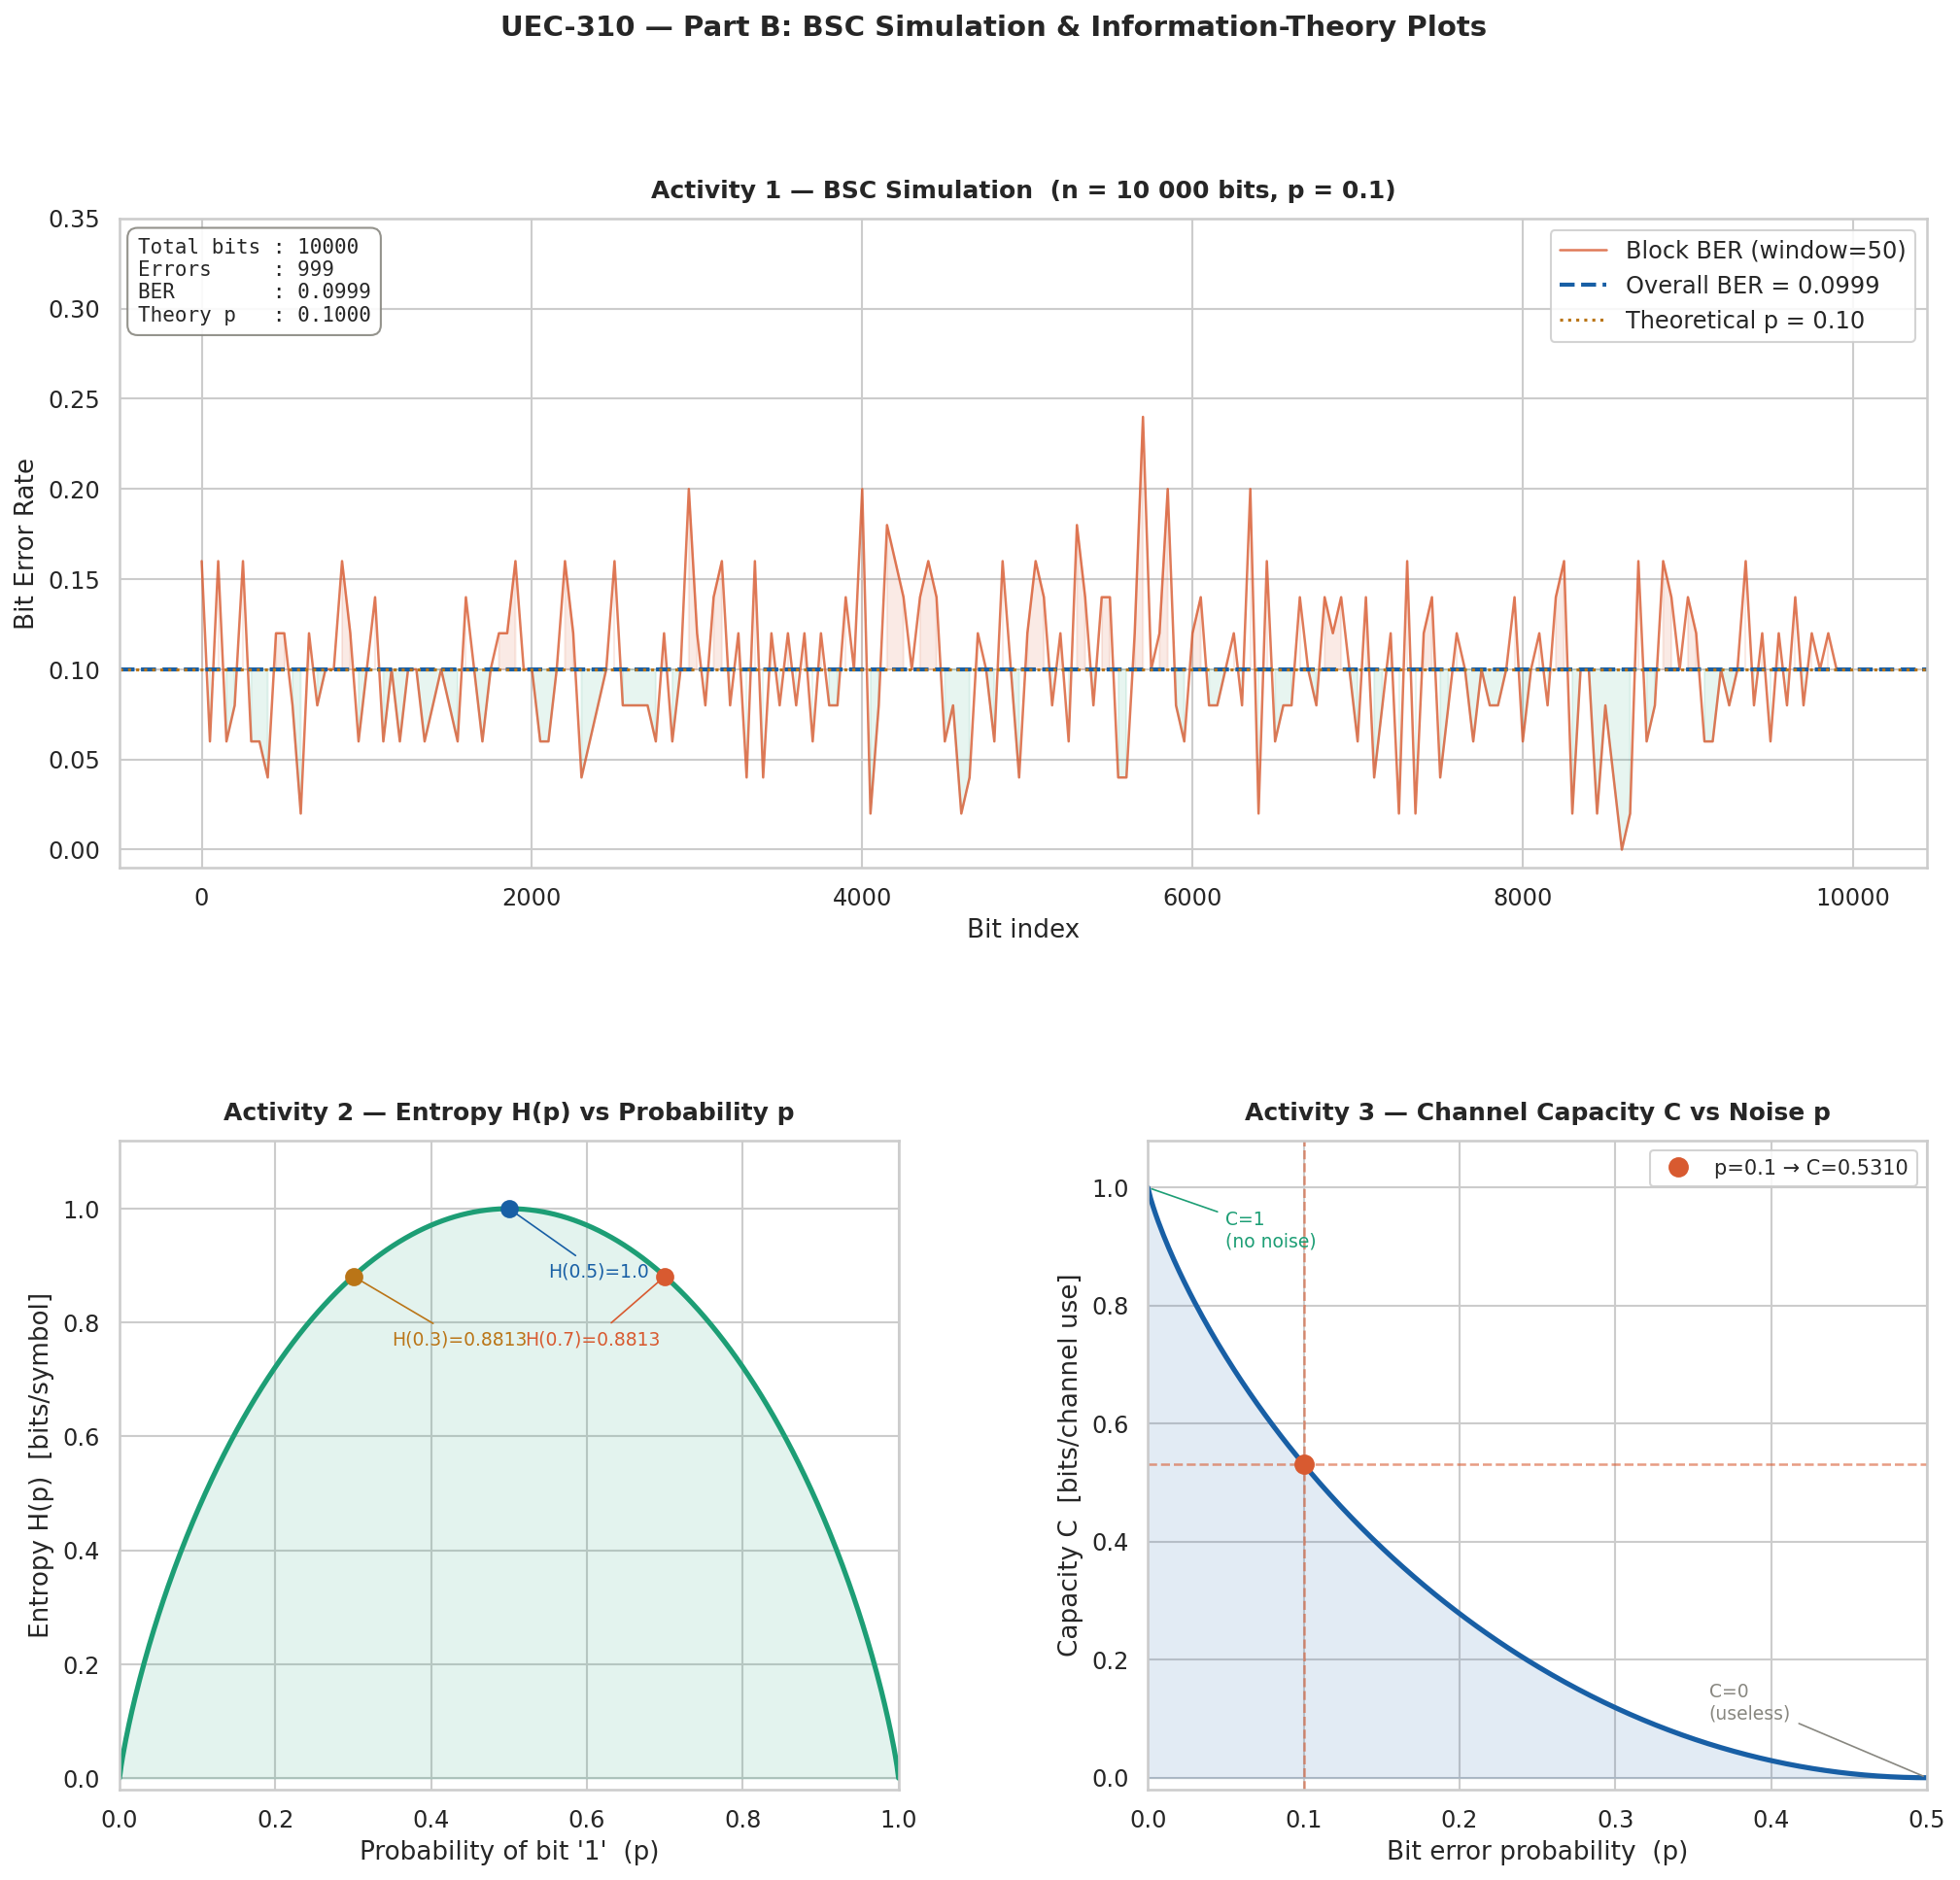
\includegraphics[width=0.98\textwidth]{b_plots.png}
\end{figure}

\begin{blueNote}
\textbf{Discussion.} The BER trace fluctuates locally across blocks of bits, but its mean remains very close to the theoretical error probability of $0.1$. The entropy curve peaks at $p=0.5$, confirming that uncertainty is maximum for an unbiased binary source. The capacity curve decreases monotonically with noise and reaches zero at $p=0.5$, where the BSC becomes useless for reliable communication.
\end{blueNote}

\section*{Conclusion}
The report shows a clear agreement between theory and simulation. Part A establishes that the source is compressible, the given coding scheme is not optimal, and the BSC capacity at $p=0.1$ is $0.5310$ bits/channel use. Part B verifies these results computationally through a reproducible Python implementation and visually interpretable plots.

\end{document}
